\cotefile{1}
\scanpage{65}
% archive sheet number: 66
troisième espace de Hilbert, si $u\in L(E,F)$, $v\in L(F,G)$, alors on aura

\[
(\overset{n}{\Lambda}v)(\overset{n}{\Lambda}u)=\overset{n}{\Lambda}(v\circ u).\tag*{(10)}
\]

Notons aussi la formule

\[
\begin{aligned}
&\deleted{\unsure{(\overset{n}{\Lambda}u)^*=\overset{n}{\Lambda}u^*}}\\
&\left\{\begin{aligned}
(u_1\wedge\ldots\wedge u_n)^*&=u_1^*\wedge\ldots\wedge u_n^*\\
(\overset{n}{\Lambda}u)^*&=\overset{n}{\Lambda}(u^*)
\end{aligned}\right.
\end{aligned}\tag*{(11)}
\]

\deleted{La première}

Pour l'établir, on peut p. ex. \deleted{partir \unsure{de la formule de polarisation}} \deleted{se borner au cas où \unsure{les $u$ sont} \unsure{supposant} (car $u_1\wedge\ldots\wedge u_n$ s'exprime \unsure{de façon naturelle} comme combinaison linéaire de \unsure{puissances} $\overset{n}{\Lambda}u$, où $u$ est une somme} partir \deleted{\unsure{du}} (car $u_1\wedge\ldots\wedge u_n=\frac1{n!}\deleted{\unsure{\sum_{p=0}^{n}(-1)^p}}\sum_{\substack{\deleted{\unsure{\sum(i_1,\ldots,i_p)}}\\0\leq p\leq n\\1\leq i_1\unsure{,\ldots,|<\ldots<}i_{\unsure{n-p|p}}\leq n}}(-1)^p\deleted{\unsure{a|q}}\overset{n}{\Lambda}(u_{i_1}+\ldots+u_{i_{n-p}})$ -- voir Introduction, 2, formule (8,--) ), où on a

\[
\begin{aligned}
((\overset{n}{\Lambda}u)\circ a_1\wedge\ldots\wedge a_n,b_1\wedge\ldots\wedge b_n)&=\det((u.a_i,b_j))=\deleted{\unsure{d}}\det((a_i,u^*b_j))\\
&=(a_1\wedge\ldots\wedge a_n,(\overset{n}{\Lambda}u^*).\,b_1\wedge\ldots\wedge b_n),
\end{aligned}
\]

ce qui établit \deleted{que} la deuxième formule (11).

En particulier, supposons $E=F$, alors on voit que l'application $u\longrightarrow\overset{n}{\Lambda}u$ de $L(E,F)$ dans $L(\overset{n}{\Lambda}^{(2)}E,\overset{n}{\Lambda}^{(2)}F)$ est \uline{multiplicative} (formule (10)) \uline{commute avec l'opération $*$} (formule 11) \inserted{elle transforme donc hermitien en hermitien,} \deleted{\unsure{si|De} \illegible{1}} plus elle transforme \deleted{\unsure{le}} un hermitien \uline{positif} $h$ en un hermitien positif, et on a, pour \deleted{\unsure{tout|$\Lambda$}} un exposant \deleted{\unsure{réel}} $\alpha>0$

\[
(\overset{n}{\Lambda}h)^\alpha=\overset{n}{\Lambda}(h^\alpha)\qquad(h\in L(E),\ h\geq0)\tag*{(12)}
\]

En effet, si $h$ est positif, on a $h=k^2$, où $k$ est un hermitien positif, d'où $(\overset{n}{\Lambda}h)=\overset{n}{\Lambda}k^2=(\overset{n}{\Lambda}k)^2$, où $\overset{n}{\Lambda}k$ est hermitien \deleted{(car \unsure{l'application} \illegible{2}}
\scanpage{66}
% archive sheet number: 67
\deleted{transforme hermitiens en hermitiens)}. Il s'ensuit bien que $\overset{n}{\Lambda}h$ \deleted{est}, \unsure{comme|carré} \unsure{d'un} hermitien, est hermitien \uline{positif}.

Enfin, la formule \unsure{(11)|(12)} est vraie si $\alpha$ est entier, elle est aussi vraie si $\alpha=\frac1n$ ($n$ entier $>0$) car on a $\bigl(\overset{n}{\Lambda}h^{1/n}\bigr)^n=\overset{n}{\Lambda}\bigl((h^{1/n})^n\bigr)=\overset{n}{\Lambda}h$, \deleted{et on voit que} \inserted{$\overset{n}{\Lambda}h^{1/n}$ est un} \uline{hermit.} \uline{positif}, il en résulte que c'est bien la racine $n^{\text{ième}}$ de $\overset{n}{\Lambda}h$. \deleted{Par suite, que (12) est \deleted{\unsure{vrai}} vraie pour le \unsure{fractionnaire},} En combinant on voit que (12) est vraie pour $\alpha$ fractionnaire.

D'autre part, si $H$ est un \deleted{\unsure{hermitien}}\inserted{\uline{opérateur}} positif dans un espace de Hilbert, on sait que $\alpha\longrightarrow H^\alpha$ est une fonction \unsure{continue|continûment} de $\alpha>0$. \deleted{\unsure{à}} Donc, l'application $\unsure{U|u}\longrightarrow\overset{n}{\Lambda}u$ de $L(E)$ dans $L(\overset{n}{\Lambda}^{(2)}E)$ étant aussi continue, on voit que les fonctions $(\overset{n}{\Lambda}h)^\alpha$ et $\overset{n}{\Lambda}(h^{\unsure{1/\alpha|\alpha}})$ sont fonctions continues de $\alpha$, \deleted{et} comme elles sont égales pour des valeurs rationnelles, elles sont égales partout, ce qui achève d'établir (12). Résumons l'essentiel de ces résultats

\uline{Proposition} 1 Soient $E$ et $F$ deux espaces de Hilbert, soient $u_i$ \deleted{\unsure{$(u_1,\ldots,u_n)$}} \inserted{$(i=1,\ldots n)$} des opérateurs linéaires continus de $E$ dans $F$, alors $u_1\wedge\ldots\wedge u_n$ est continu pour les structures préhilbertiennes de $\overset{n}{\Lambda}^{\unsure{a|q}}E$ et $\overset{n}{\Lambda}^{a}F$, et se prolonge donc par continuité en une application linéaire continue de $\overset{n}{\Lambda}^{\unsure{(1)|(2)}}E$ dans $\overset{n}{\Lambda}^{(2)}F$, \deleted{\unsure{et}} c. à d. un $u_1\wedge\ldots\wedge u_n$, \deleted{et satisfait à} de norme $\leq\lVert u_1\rVert\ldots\lVert u_n\rVert$.

L'application $u\longrightarrow\overset{n}{\Lambda}u$ de $L(E)$ dans $L(\overset{n}{\Lambda}^{(2)}E)$ est multiplicative, commute à l'opération $*$, transforme op. hermitiens en op. hermitiens et opérateurs positifs en
\scanpage{67}
% archive sheet number: 68
\margin{\unsure{à mettre au net|à mettre au point|à mettre après} Weyl \unsure{sur les propriétés} dans les \unsure{Hilbert|hilbertiens}}

% margin note written sideways
\margin{à \unsure{développer} en rédigeant le cas de la dimension finie}

% margin note written sideways
\margin{\deleted{\uline{\unsure{Conséquences|Conséquence}, \unsure{changement de notation}.} Pour la suite, les \unsure{notations} suivantes seront utiles. Si $u$ est un op. compact dans un espace de Hilbert complexe, on désigne par $(\lambda_i(u))$ la suite des valeurs propres de $u$ \unsure{répétées|ordonnées|comptées} suivant leurs multiplicités, \deleted{\unsure{de}} rangées de façon que \unsure{la suite en module|leur suite en module} soit décroissante. Si \unsure{cette liste} ne \unsure{contient} qu'un nombre fini de valeurs propres non nulles, on complète par suite \deleted{\unsure{d'une infinité de valeurs nulles}}, en posant \unsure{$\lambda_i(u)=0$ pour les autres $i$}. Si $u$ est un op. compact \illegible{2}, \unsure{$(\rho_i(u)=(\lambda_i((u^*u)^{1/2}))$|$\rho_i(u)=(\lambda_i(uu^*u)^{1/2})$}, suite \inserted{décroissante} des valeurs propres de $(u^*u)^{1/2}$ (qui est la même que celle des valeurs \unsure{propres} de $(uu^*)^{1/2}$). \deleted{\unsure{La définition doit s'étendre}} \unsure{Si $u$ est unitaire} \illegible{2}. On obtient \unsure{ainsi tout naturellement}, en \unsure{liaison} avec les notations. Si \unsure{donc} $u$ est un op. compact positif d'un \unsure{espace}, $\lambda_i(u)=\rho_i(u)=\unsure{\sigma_i(u)}$.}}

\deleted{\unsure{Supposons}}

\uline{Proposition 2} \deleted{\unsure{Si $u$ est un}} Soit $u$ un op. compact dans l'espace hilbertien complexe \deleted{\unsure{H}}$E$, $(\lambda_i)$ la suite de ses valeurs propres. \deleted{\unsure{comprises}} Alors \deleted{les valeurs} $\overset{n}{\Lambda}u$ est un op. compact dans $\overset{n}{\Lambda}^{(2)}E$, ayant \inserted{exactement} le \unsure{système} de valeurs propres \deleted{\unsure{les valeurs|propres}} $\lambda_{i_1}\ldots\lambda_{i_n}$, avec $i_1<i_2<\ldots<i_n$.

Comme l'application $\deleted{\unsure{E|F}}u\longrightarrow\overset{n}{\Lambda}u$ \deleted{est une \unsure{appl.}} de $L(E)$ dans $L(\overset{n}{\Lambda}^{\unsure{(2)|(1)}}E)$ est continue, \deleted{si $u$ est compact, il est La question de \unsure{rang f|rang fini}} et transforme les opérateurs de rang fini en opérateurs de rang fini, il s'ensuit que si $u$ est compact, donc limite d'opérateurs de rang fini, \deleted{il en est de même} \inserted{alors} $\overset{n}{\Lambda}u$ est aussi limite d'opérateurs de rang fini, donc aussi un op. compact.

D'autre part, si $u$ est de rang fini, \deleted{il \unsure{peut} se mettre sous forme d'un} \deleted{\inserted{qui à une base hilb., si $u$ \unsure{commutait|convenable}} \unsure{certain} \unsure{espace} \unsure{tel} dont un nb fini seulement, \inserted{\unsure{Alors} soit $N$, un \unsure{tel}, considérons} soit $E_1$ l'espace} soit $E_{1}$ l'intersection de son noyau $\unsure{u^{-1}(0)|u^{-1}0}$ avec l'orthogonal de \unsure{l'image} $u(E)$, et soit $E_0$ l'orthogonal de $E_1$.

Alors $u$ \uline{s'annule} sur $E_1$, et $u(E)\subset E_0$, donc $u$ \uline{\unsure{conserve|invarie}} $E_0$. $\overset{n}{\Lambda}E$ est \deleted{la somme \unsure{di}} \inserted{algébriquement} isomorphe à la somme $\sum_{0\leq p\leq n}\overset{n-p}{\Lambda}E_0\otimes\overset{p}{\Lambda}E_1\deleted{\unsure{\}}}$, et quand on munit d'une \deleted{\unsure{$E$|$F$|$\Lambda E$}} part $\overset{n}{\Lambda}E$ de sa structure préhilbertienne, et d'autre part $\overset{n-p}{\Lambda}E_0$ et $\overset{p}{\Lambda}E_1$ de leur structure préhilbertienne naturelle, donc sur $\overset{n-p}{\Lambda}E_0\otimes\overset{p}{\Lambda}E_1$ une structure préhilbertienne naturelle, on vérifie que l'isomorphisme $\overset{n}{\Lambda}E=\sum_{\unsure{0\leq p\leq n}}\overset{n-p}{\Lambda}E_0\otimes\overset{p}{\Lambda}E_1$
\scanpage{68}
% archive sheet number: 69
conserve ces structures préhilbertiennes \deleted{et} Noter que à une décomposition de $E$ \deleted{\unsure{en somme directe}} en somme de \unsure{sous-espaces} mutuellement orthogonaux $E_0$ et $E_1$ donne une décomposition orthogonale

\[
\overset{n}{\Lambda}^{(2)}E=\sum_{0\leq p\leq n}\overset{n-p}{\Lambda}^{(2)}E_0\overset{(2)}{\otimes}\overset{p}{\Lambda}^{(2)}E_1 .
\]

Si $u$ est un op. dans $E$ s'annulant sur $E_1$, alors on a $(\overset{n}{\Lambda}u).(x_1\wedge\ldots\wedge x_n)\inserted{=ux_1\wedge\ldots\wedge ux_n}=0$, \deleted{\unsure{pourvu|puisque}} dès que l'un \deleted{\unsure{des}} des $x_i$ \deleted{\unsure{dans} $\overset{n}{\Lambda}$} $\unsure{\in E_1}$, donc $\overset{n}{\Lambda}u$ s'annule sur \deleted{\unsure{le}} toutes les \deleted{\unsure{composantes}} \inserted{termes composants} de $\sum_p\overset{n-p}{\Lambda}E_0\otimes\overset{p}{\Lambda}E_1$ sauf le premier, \deleted{et si de même \unsure{soit}}

il en résulte par prolongement par continuité que l'op. correspondant dans $\overset{n}{\Lambda}^{(2)}E$ s'annule sur tous les $\overset{n-p}{\Lambda}^{(2)}E_0\overset{(2)}{\otimes}\overset{\unsure{p|0}}{\Lambda}^{(2)}E_{\unsure{1|i}}$, \deleted{\unsure{sauf}} avec $p\neq0$. \deleted{\unsure{De}} \inserted{On voit de} même que, si $u$ \unsure{invarie|conserve} $E_0$, alors $\overset{n}{\Lambda}u$ conserve $\overset{n}{\Lambda}^{(2)}E_0$, de plus dans \deleted{\unsure{cet}} \deleted{\unsure{esp}} ce dernier espace, il se réduit à

$\overset{n}{\Lambda}v$, où $v$ est la restriction de $u$ à $E_0$. Dans le cas actuel, \deleted{\illegible{2}} \inserted{($u(E_1)=0$, $u(E_0)\subset E_0$, \deleted{\unsure{de|et}} $E_0$ de dim. finie)} on voit donc que \deleted{\unsure{$\overset{n}{\Lambda}u$ se ramène}} les valeurs propres de $\overset{n}{\Lambda}u$ dans $\overset{n}{\Lambda}^{(2)}E$, sont les valeurs propres de $\overset{n}{\Lambda}v$ dans $\uline{\overset{n}{\Lambda}^{(2)}E_0}=\overset{n}{\Lambda}E_0$. Il est bien connu, que

\deleted{\unsure{si est de}} \deleted{\unsure{ce}} puisqu'il s'agit d'opérateurs dans l'espace vectoriel de dim. finie $E_0$, que ces valeurs propres s'obtiennent en \deleted{\unsure{prenant}} \inserted{tous} les produits \inserted{de $n$} \deleted{\unsure{au}} valeurs propres de $v$ correspondant à des indices \unsure{distincts|deux à deux distincts} (on le voit par ex en mettant $v$ sous forme de matrice triangulaire\unsure{?|/}\unsure{ainsi|supér.}), et
\scanpage{69}
% archive sheet number: 70
que d'autre part les valeurs propres non nulles de $u$ et de sa restriction $v$ à $E_0$ sont les mêmes, la prop. 3 est \unsure{par|donc} là démontrée pour les op. $u$ de rang fini.

Comme on sait que le système \deleted{\unsure{tout}} entier, propre à un op. compact $u$ dans un espace de Banach, dépend \deleted{\unsure{continûment}} \unsure{continûment} \deleted{\unsure{pris comme un}} (dans un sens évident à préciser) de $u$, il s'ensuit que la prop. 3 est aussi vraie pour toute limite d'opérateurs de rang fini, i.e. pour tous les op. compacts.

On conclut de la prop. 3 les résultats suivants, qui seront essentiels au N\textsuperscript{o} suivant : \deleted{\unsure{(lettre Hubert|(cette thèse} \unsure{pour} \illegible{2}}

\uline{Corollaire 2} Soit $u$ un op. \inserted{compact} dans un espace de Hilbert complexe $E$, \inserted{alors pour tout entier $n\geq1$, on a} \deleted{soit $(\lambda_i)$ la suite de ses valeurs propres non nulles, \unsure{chaque} \illegible{2} \unsure{pour} tout \unsure{$u\in L(E)$}, \unsure{$\lambda_i(\Lambda^n)$} pour un entier $n$, soit \unsure{$(\rho_i)$} la suite décroissante des valeurs propres de l'adjoint. Alors pour tout $n$ \unsure{on a}}

\[
|\lambda_1\ldots\lambda_n|\leq\rho_1\ldots\rho_n\tag*{(23)}
\]

\margin{au \uline{N\textsuperscript{o} 1}}

Voir conventions de notation \deleted{avant la prop 3} \inserted{au N\textsuperscript{o} 1}

En effet, d'après la \deleted{prop. 3 le \unsure{terme} est la plus grande des valeurs propres de} \inserted{\unsure{formule ci-contre} (23)} le premier membre est ég. à \deleted{\unsure{$\lambda_1$}} $|\lambda_1(\overset{n}{\Lambda}u)|$, donc \unsure{maj.} par $\lVert\overset{n}{\Lambda}u\rVert$, \deleted{\unsure{d'o}} ce qui n'est autre que le deuxième mb de (23), en vertu de (22).

\deleted{$\lVert\overset{n}{\Lambda}u\rVert=\lVert((\overset{n}{\Lambda}u)^*(\overset{n}{\Lambda}u))^{1/2}\rVert=\deleted{\unsure{(\overset{n}{\Lambda}(u^*u))^{1/2}}}\lVert\overset{n}{\Lambda}h\rVert$, où $h=(u^*u)^{1/2}$ (prop 1), or, $\lVert\overset{n}{\Lambda}h\rVert$ est \inserted{$\overset{n}{\Lambda}h$ étant hermitien positif, \unsure{par suite}} la plus grande des valeurs propres de $\overset{n}{\Lambda}h$, donc à $\rho_1\ldots\rho_n$ d'après (21).}

\uline{Corollaire 3} Soient \deleted{\unsure{$u$ et $v$ des op. compacts dans un}} \inserted{$E,F,G$ trois espaces de Hilbert,}

% margin note written sideways
\margin{\uline{Corollaire 1} Soit $u$ \deleted{un op. compact de l'un deux} \inserted{opérateur compact} de \inserted{$E$ dans un autre $F$} \unsure{espace} de Hilbert \deleted{\unsure{complexe}}, on a pour tout entier $\geq1$ \inserted{si $E=F$}}

% margin note written sideways
\margin{$\text{(21)}\quad\lambda_1(u)\ldots\lambda_n(u)=\lambda_1(\overset{n}{\Lambda}u)$}

% margin note written sideways
\margin{et dans tous les cas, on a $\text{(22)}\quad\rho_1(u)\ldots\rho_n(u)=\lVert\overset{n}{\Lambda}u\rVert$}

% margin note written sideways
\margin{\deleted{\unsure{on pose}} pour les notations, voir \unsure{la rédaction} qui précède la prop. 3). En effet, la formule (21) est une \unsure{conséquence} \unsure{immédiate} de la prop. 3. Quant à la formule (22), on note que $\rho_i(u)^2=\lambda_i(u^*u)$, donc le \unsure{carré du} premier mb de (22) est en vertu de (21), égal à}

% slanted
\margin{$\lambda_1(\overset{n}{\Lambda}(u^*u))=\unsure{\rho_1|\lambda_1}((\overset{n}{\Lambda}u)^*\overset{n}{\Lambda}u)$ (\unsure{prop. 2} Voir \deleted{\illegible{2}}) $=\lVert\overset{n}{\Lambda}u\rVert^2$ \unsure{(facteurs $\rho$} \unsure{$h=\, $} \illegible{2}}
\scanpage{70}
% archive sheet number: 71
\deleted{espace de Hilbert $H$,} soit $u$ un op. compact de $E$ dans $F$, $v$ un op. \unsure{cpt|cpct} de $F$ dans $G$, \deleted{posons $w=vu$. Soit $(\rho_i(w))$ la suite des valeurs propres de $\sqrt{w^*w}$} Alors, pour tout entier $n\geq1$, on a

\[
\rho_1(uv)\ldots\rho_n(uv)\leq(\rho_1(u)\rho_1(v))\ldots(\rho_n(u)\rho_n(v))\tag*{(24)}
\]

\deleted{En effet, \deleted{il est \unsure{aisé}} \deleted{$\rho_1(uv)\ldots\rho_n(uv)$} c'est évident pour $n=1$, car on a de façon générale $\rho_1(w)=\lVert(w^*w)^{1/2}\rVert=\lVert w\rVert$, et la formule se réduit donc à $\lVert uv\rVert\leq\lVert u\rVert\lVert v\rVert$. Dans le cas général, on a, puisque \deleted{\unsure{$\rho_1(uv)$}} \deleted{\unsure{ce qui}} \deleted{\unsure{Et}} $\rho_i(w)^2=\rho_i(w^*w)$ pour \deleted{tout} op. compact $w$ :}

\[
\begin{aligned}
\deleted{(\rho_1(uv)\ldots\rho_n(uv))^2}&\deleted{=\lambda_1((uv)(\unsure{uv|vu})^*)\ldots\lambda_n((uv)(\unsure{uv|vu})^*)=}\\
&\deleted{\lambda_1(\overset{n}{\Lambda}(uv)(uv)^*)\unsure{\leq}=\lambda_1}
\end{aligned}
\]

En effet, en vertu de \deleted{\unsure{form.}} (23), le premier mb est égal à $\lVert\overset{n}{\Lambda}(uv)\rVert$, i.e. $\lVert(\overset{n}{\Lambda}u)(\overset{n}{\Lambda}v)\rVert$, \deleted{\unsure{(prop 1)}} donc majoré par $\lVert\overset{n}{\Lambda}u\rVert\,\lVert\overset{n}{\Lambda}v\rVert$, qui n'est autre que le deuxième mb de (24) en vertu de (23).

L'idée de la démonstration de (13) et (14) sont dues à H. Weyl, ainsi que leur utilisation pour les inégalités de convexité des \unsure{fonct.|fonctions|formes}, au \deleted{\S} N\textsuperscript{o} suivant.
\scanpage{71}
% archive sheet number: 72
\unsure{5.)|5,)|3.} Puissances extérieures d'op. de Fredholm, inégalités diverses.

\uline{Prop. 1}

\[
\lVert u_1\wedge\ldots\wedge u_n\rVert_1\leq\frac1{n!}\lVert u_1\rVert_1\ldots\lVert u_n\rVert_1\tag*{\textcircled{1}}
\]

\uline{Corollaire 1}

\[
\left\{\begin{aligned}
\alpha_n(u_1,\ldots,u_n)&=\operatorname{Tr}(u_1\wedge\ldots\wedge u_n)\\
\alpha_n(u)&=\operatorname{Tr}\overset{n}{\Lambda}(u)
\end{aligned}\right.\tag*{$\substack{\text{\textcircled{2}}\\\text{\textcircled{3}}}$}
\]

\uline{Corollaire 2}

\[
|\alpha_n(u_1\deleted{\unsure{,\ldots}},\ldots,u_n)|\leq\frac1{n!}\lVert u_1\rVert_1\ldots\lVert u_n\rVert_1\quad\text{en particulier }\ |\alpha_n(u)|\leq\frac1{n!}\lVert u\rVert_1^n\tag*{(4)}
\]

\[
\deleted{(5)\quad|\alpha_n(u)|\leq\frac1{n!}\lVert u\rVert^{\unsure{n|2}}}
\]

\deleted{\uline{Corollaire 3}}

\[
\begin{aligned}
\deleted{(6)\quad\lVert\overset{n}{\Lambda}u\rVert_1}&\deleted{=\alpha_n(|u|)}\\
\deleted{(7)\quad\lVert\overset{n}{\Lambda}u\rVert_1}&\deleted{=\sqrt{\alpha_n(u^*u)}}
\end{aligned}
\]

\[
\deleted{\bigl(|\alpha_n(u)|\leq\lVert\overset{n}{\Lambda}u\rVert_1=\alpha_n(|u|)\leq\frac1{n!}\lVert u\rVert_1^n\bigr)}
\]

\deleted{\uline{Corollaire 4}}

\[
\deleted{(8)\quad\alpha_n(u)\leq\alpha_n(|u|)}
\]

\uline{Corollaire 3}

\[
|\alpha_n(u)|\leq\deleted{\unsure{\alpha_n u}}\alpha_n(|u|)=\lVert\overset{n}{\Lambda}u\rVert_1\leq\frac1{n!}\lVert u\rVert_1^n\tag*{\textcircled{5}}
\]

Car \unsure{a|on a} $|\alpha_n(u)|\leq\lVert\overset{n}{\Lambda}u\rVert_1$ en vertu de (3), et $\alpha_n(|u|)=\operatorname{Tr}(\overset{n}{\Lambda}(|u|))=\operatorname{Tr}|\overset{n}{\Lambda}u|=\lVert\overset{n}{\Lambda}u\rVert_1$ (deux références) enfin $\lVert\overset{n}{\Lambda}u\rVert_1\leq\frac1{n!}\lVert u\rVert^n$ (formule (1))

\margin{?}

\deleted{\uline{Corollaire \unsure{4|3}}}

\[
\deleted{(6)\quad\left\{\begin{aligned}
\lVert\overset{n}{\Lambda}u\rVert_1&=\alpha_n(|u|),\\
\lVert\overset{n}{\Lambda}u\rVert_{\unsure{2|1}}&=\sqrt{\alpha_n(u^*u)}
\end{aligned}\right.}
\]

\uline{Corollaire 4}

\[
|\det(1+u)|=\det(1+|u|)\tag*{\textcircled{6}}
\]

\uline{Théorème 1} Si $u\in L^1(E)$, alors \deleted{$\det(1+zu)$} $(\lambda_i(u))\in l^1$, et $\det(1+zu)$ est de \uline{genre} $0$ :

\[
\det(1+zu)=\prod_i(1+z\lambda_i(u))\tag*{\textcircled{7}}
\]

Équivaut à

\[
\begin{aligned}
\alpha_n(u)&=\sum_{i_1<\ldots<i_n}\lambda_{i_1}(u)\ldots\lambda_{\unsure{n i_n|i_n}}(u)\\
\operatorname{Tr}u&=\sum_i\lambda_i(u)
\end{aligned}\tag*{$\substack{\text{\textcircled{8}}\\\text{\textcircled{9}}}$}
\]

Implique

\[
\alpha_n(|u|)=\lVert\overset{n}{\Lambda}u\rVert_1=\sum_{\unsure{i_1<\ldots<i_2|i_1<\ldots<i_n}}\rho_{i_1}(u)\ldots\rho_{i_n}(u)\tag*{\textcircled{10}}
\]

\margin{\unsure{Ce qui revient|Ce qui est} \deleted{\unsure{au|un}} dont résulte de nouveau \unsure{(8) en l'appliquant|(8) en l'étendant} à $\overset{n}{\Lambda}u$.}

Pour la preuve, on \deleted{est} ramènera au cas où $u$ est hermitien positif, où c'est facile,

\uline{Prop 2}

\[
\deleted{\unsure{\lVert u_1\wedge v_1\wedge u\rVert} \lVert(\overset{p_1}{\Lambda}u_1)\wedge\ldots\wedge(\overset{p_k}{\Lambda}u_k)\rVert_1\leq\lVert\overset{p_1}{\Lambda}u_1\rVert_1\ldots\lVert\overset{p_k}{\Lambda}u_k\rVert}
\]

\[
\lVert(\overset{p}{\Lambda}u)\wedge(\overset{q}{\Lambda}v)\rVert_1\leq\frac{p!q!}{(p+q)!}\lVert\overset{\unsure{p|0}}{\Lambda}u\rVert_1\lVert\overset{q}{\Lambda}v\rVert_1=\frac{p!q!}{(p+q)!}\alpha_p(|u|)\alpha_q(|v|)\tag*{\textcircled{11}}
\]

(le même vrai pour plus de deux facteurs, l'écriture $(\overset{p}{\Lambda}u)\wedge(\overset{q}{\Lambda}v)$ est ici \uline{\unsure{mnemotechnique|mnémotechnique}}).
\scanpage{72}
% archive sheet number: 73
Soit

\[
\begin{aligned}
u&=\sum\rho_i\bar b_i\otimes a_i & \rho_i&=\rho_i(u)\quad\text{etc}\\
v&=\sum\sigma_j\bar d_j\otimes c_j & \sigma_j&=\sigma_j(v)
\end{aligned}
\]

d'où

\[
\begin{aligned}
(\overset{p}{\Lambda}u)\wedge(\overset{q}{\Lambda}v)
&=\frac1{(p+q)!}\sum_{\substack{i_1\ldots i_p\\j_1\ldots j_q}}\rho_{i_1}\ldots\rho_{i_p}\sigma_{j_1}\ldots\sigma_{j_q}
\overline{b_{i_1}\wedge\ldots b_{i_p}\wedge d_{j_1}\wedge\ldots d_{j_q}}\otimes\\[-2pt]
&\hspace{25mm}(a_{i_1}\wedge\ldots a_{i_p}\wedge c_{j_1}\ldots c_{j_q})
\end{aligned}
\]

On peut sommer sur des ($i_\alpha$) tous distincts et des ($j_\beta$) tous distincts, soit

donc

\[
\begin{aligned}
\lVert(\overset{p}{\Lambda}u)\wedge(\overset{q}{\Lambda}v)\rVert_1
&\leq\frac{1}{(p+q)!}p!q!\sum_{\substack{i_1<\ldots<i_p\\j_1<\ldots<j_q}}\rho_{i_1}\ldots\rho_{i_p}\sigma_{j_1}\ldots\sigma_{j_q}\\
&=\frac{p!q!}{(p+q)!}\left(\sum_{i_1<\ldots<i_p}\rho_{i_1}\ldots\rho_{i_p}\right)
\left(\sum_{j_1<\ldots<j_q}\sigma_{j_1}\ldots\sigma_{j_q}\right)
=\frac{p!q!}{(p+q)!}\lVert\overset{p}{\Lambda}u\rVert_1\lVert\overset{q}{\Lambda}v\rVert_1 .
\end{aligned}
\]

\uline{Corollaire 1} Si $u,v\in L^1(E,F)$, alors \deleted{\unsure{soit}} pour $r\geq0$

\[
\deleted{\det}\det(1+\deleted{\unsure{r}}r|u+v|)\leq\det(1+r|u|)(\det(1+r|v|))\tag*{\textcircled{12}}
\]

i.e. on a

\[
\prod_i(1+r\rho_i(u+v))\leq\left(\prod_i1+r\rho_i(u)\right)\left(\prod_i(1+r\rho_i(v))\right)\tag*{\textcircled{13}}
\]

On va \unsure{même|en} montrer que l'on a majoration coëfficient par coëfficient, donc que

\uline{Corollaire 2} Pour tout $n$,

\[
\alpha_n(|u+v|)\leq\sum_{0\leq\underline{p}\leq n}\alpha_p(|u|)\alpha_{n-p}(|v|)\tag*{\textcircled{14}}
\]

En effet, on a \deleted{$|u+v|=U(u+v)$, où $U\in L(E,E)$, $\lVert U\rVert\leq1$, donc $\alpha_n(|u+v|)=\lVert\overset{n}{\Lambda}U(u+v)\rVert_1=\overset{n}{\Lambda}U\,\overset{n}{\Lambda}(u+v)$} \inserted{$\alpha_n(|u+v|)=\lVert\overset{n}{\Lambda}(u+v)\rVert_1$}

\[
\begin{aligned}
\overset{n}{\Lambda}(u+v)&=\sum_{p=0}^n\frac{n!}{p!(n-p)!}(\overset{p}{\Lambda}u)\wedge(\overset{n-p}{\Lambda}v)\qquad\text{d'où}\\
\alpha_n(|u+v|)\ \lVert\overset{n}{\Lambda}(u+v)\rVert_1
&\leq\sum_{p=0}^n\frac{n!}{p!(n-p)!}\lVert(\overset{p}{\Lambda}u)\wedge(\overset{n-p}{\Lambda}v)\rVert_1\leq\sum\deleted{\unsure{\frac{n!}{p!(n-p)!}}}\deleted{\unsure{p!q|\frac{p!(n-p)!}{n!}}}\alpha_{\unsure{n|p}}(|u|)\alpha_{n-p}(|v|).
\end{aligned}
\]

\unsure{Prouvons|Prouver} le

\uline{Théorème 2} Pour $u,v\in L_0(E,F)$, \inserted{$r\geq0$} et pour \deleted{tout} $\unsure{m|n}$, on a

\[
\prod_1^m(1+r\rho_i(u+v))\leq\left(\prod_1^m(1+r\rho_i(u))\right)\prod_1^m(1+r\rho_i(v))\tag*{\textcircled{15}}
\]

De façon plus précise, on a majoration coëfficients par coëfficients, i.e. pour \deleted{tout} entier \deleted{\unsure{$m$}} \unsure{$m$}, $0\leq m\leq n$, on a

\[
\deleted{\unsure{S_n^m(u+v)=\sum_{p=0}^{m}|S_n^m(u+v)\leq\sum_{p\leq\ldots}^{m}}}
\]

\[
\sigma_{\deleted{\unsure{p}}n}^{m}(u+v)\leq\sum_{p=0}^m\sigma_n^p(u)\,\sigma_{\unsure{n|\text{--}}}^{m-p}(v)\tag*{\textcircled{16}}
\]

% slanted
\margin{\uline{notation \unsure{?|$\leq0$}} à \uline{réviser}}

où de façon générale on pose, pour \inserted{$w\in L_0(E,F)$ et} $0\leq m\leq n$ :

\[
\sigma_n^m(w)=\sum_{1\leq i_1<\ldots<i_m\leq n}\rho_{i_1}(w)\ldots\rho_{i_m}(w)\tag*{\textcircled{17}}
\]

Comme \unsure{cas|en} particulier \unsure{des|aux} formules (16), pour $\unsure{v|p|m|n}=1$, signalons \inserted{\textcircled{18}}
\scanpage{73}
% archive sheet number: 74
On va prouver la proposition auxiliaire

\uline{Prop 3} On a, pour $u\in L_0(E,F)$, et $0\leq m\leq n$

\[
\sigma_n^m(u)=\operatorname{Sup}_{\left\{\substack{v_n\in L(F,E)\\\lVert v_n\rVert\leq1\\\operatorname{rang}v_n\leq n}\right.}|\alpha_m(v_nu)|=\operatorname{Sup}_{\unsure{v_n|v}}\{\alpha_{\unsure{n|m}}(|v_nu|)\tag*{\textcircled{19}\ \deleted{\textcircled{18}}}
\]

\deleted{\unsure{En effet}.}

En effet, prouvons \deleted{que $|\alpha_m(v_nu)|=|\operatorname{Tr}\overset{m}{\Lambda}v_nu|\leq$} \deleted{Il suffit} pour prouver l'inégalité \deleted{$|\operatorname{Tr}(\overset{m}{\Lambda}v_n)(\overset{m}{\Lambda}u)|\leq\lVert\overset{m}{\Lambda}\unsure{v_n}\rVert\,\lVert\overset{m}{\Lambda}u\rVert_1\leq\overset{m}{\Lambda}u$} $|\alpha_m(v_nu)|\leq\sigma_n^m(u)$, comme on a $\rho_i(v_nu)\leq\rho_i(u)$ pour tout $i$ (\unsure{---}), il suffit d'établir $|\alpha_m(v_nu)|\leq\sigma_n^m(v_nu)$, donc le

\uline{lemme} Si $u\in L(E,E)$ est de rang $\leq n$, on a $|\alpha_m(u)|\leq\{\alpha_m(|u|)\}\leq\sigma_n^m(u)$. Or on a, si $v$ est la restriction de $u$ à $u(E)$, \deleted{et $\alpha$ l'application identique $u(E)\longrightarrow E$,}

\[
|\alpha_m(\deleted{\unsure{uv}}u)|=|\alpha_m(v)|\leq\deleted{\unsure{\alpha_m(|v|)}}\sum_{1\leq i_1\ldots\leq i_m\leq n}\rho_{i_1}(\unsure{v|u|w})\ldots\rho_{i_m}(\unsure{u|v|w}),
\]

et comme \deleted{\unsure{que}} $v=\alpha^*u\alpha$ ($\alpha$ appl. identique $u(E)\longrightarrow E$) d'où $\rho_i(v)\leq\lVert\alpha^*\rVert\lVert\alpha\rVert\rho_i(u)\leq\rho_i(u)$, la formule voulue.

\margin{\unsure{1|$\uparrow$}}

\deleted{\unsure{Montrons}} Montrons que la borne en (\unsure{19|18}) est \uuline{atteinte} : on peut supposer $E$ de dimension $\geq n$, \deleted{\unsure{alors}} et si \deleted{\unsure{l'on est} $\sum_{i=1}^{\infty}$ des \unsure{$\rho_i e_i\otimes f_i$}}, $u=\sum\rho_i\bar e_i\otimes f_{\unsure{i|j|2}}$, on prend $v_n=\sum_1^n\bar f_i\otimes e_i$, d'où $v_nu=\sum_1^n\rho_i\bar e_i\otimes e_i$, et $\alpha_m(v_nu)=S_n^m(u)$ (remarque : si $F=E$, et $u$ hermitien, alors on peut prendre $v$ projecteur hermitien de rang $n$ pour $E$ de dimension $\leq n$).

Prouvons maintenant (16) : \deleted{\unsure{Or} (17) nous ramène à prouver que} \inserted{(\unsure{19|18}) nous ramène à prouver} que $|\alpha_m(w(u+v))|\deleted{\unsure{\leq\sum_{p=0}^{n}\alpha_p(wu)}}$ est majoré par le second mb pour \deleted{\unsure{tout}} $w\in L(F,E)$ telle que $\lVert w\rVert\leq1$, $\operatorname{rang}w\leq n$, \deleted{\unsure{or il est}} \deleted{\unsure{on}} on a ((14))

\[
|\alpha_{\unsure{n|m}}(w(u+v))|\leq\alpha_{\unsure{n|m}}(|wu+wv|)\leq\sum_{p=0}^{m}\alpha_p(|wu|)\alpha_{m-p}(|wv|)
\]

\deleted{d'autre part on a}

\[
\deleted{\alpha_p(|wu|)=\lVert\overset{p}{\Lambda}wu\rVert_1=\lVert(\overset{p}{\Lambda}w)(\overset{p}{\Lambda}u)\rVert_1\leq\lVert\overset{\unsure{n|p}}{\Lambda}w\rVert\,\lVert\overset{p}{\Lambda}u\rVert_1\leq\lVert\overset{\unsure{n|p}}{\Lambda}u\rVert_1=\unsure{\alpha_p(|u|)}}
\]

\deleted{or l'opération \unsure{de la}} Or (\unsure{19|18}) montre que $\alpha_p(|wu|)\leq\sigma_n^p(u)$ et $\alpha_{m-p}(|wv|)\leq\sigma_n^{m-p}(v)$, d'où la formule (18).
\scanpage{74}
% archive sheet number: 75
Le système des inégalités \textcircled{17} (pour $m,n$ variables) et \uline{la conséquence (15)} semblent les inégalités les plus fortes possibles majorant \unsure{le|les} \inserted{\unsure{système|systèmes|fonction} des} $\rho_i(u+v)$ en fonction des $\rho_i(u)$, $\rho_i(v)$. Notons qu'on pourrait déduire \deleted{\unsure{de la même façon}} \inserted{directement} l'inégalité \uline{(15)} à partir de l'inégalité \uline{(12)} qu'elle \uline{généralise}, \uline{pour cela signalons} la \deleted{\unsure{prop}}

\uline{Prop. 4} Si $u\in L_0(E,F)$, \deleted{\unsure{et}} $n$ est un entier $>0$, on a

\[
\deleted{\unsure{d|\det}}\prod_1^n(1+\rho_i(u))=\operatorname{Sup}_{\substack{v_n\in L(F,E)\\\lVert v_n\rVert\leq1\\\operatorname{rang}v_n\leq n}}\det(1+v_nu)\tag*{(18)}
\]

Cette \deleted{démonstration} \inserted{formule} se démontre comme (17), \deleted{\unsure{on peut même}} \inserted{\deleted{\unsure{par}} le} raisonnement est \deleted{m\unsure{algré} \unsure{un} peu \unsure{simple}} \inserted{laissé au lecteur}

\figure{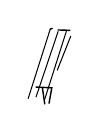
\begin{tikzpicture}[x=1mm,y=1mm,line cap=round]
\draw[line width=.13mm] (0,0)--(2.8,8.8) (1.0,.2)--(3.8,8.5) (2.1,-.1)--(4.9,8.7) (3.7,3.6)--(5.4,7.9);
\draw[line width=.18mm] (2.8,8.8)--(3.05,8.9) (3.8,8.7)--(5.3,8.65) (1.0,1.45)--(3.0,1.35)--(2.65,-.6) (1.8,1.4)--(2.1,-.7);
\end{tikzpicture}}
\scanpage{75}
% archive sheet number: 76
\[
\sum_1^n\log(1+r\rho_i(u+v))\leq\sum_1^n\log(1+r\rho_i(u))+\sum_1^n\log(1+r\rho_i(v))
\]

\[
S_{\deleted{\unsure{m}}\varphi}^{n}(u+v)\leq S_\varphi^n(u)+S_\varphi^n(v)\qquad S_\varphi^n(w)=\sum_1^n f_\varphi(\rho_i(w))
\]

\[
f_\varphi(\rho)=\int_0^{+\infty}\frac{\varphi(r)}{\frac1\rho+r}\,dr=\int_0^{+\infty}\varphi\left(\frac s\rho\right)\frac{ds}{1+s}
\]

$\varphi$ fonction décroissante

(motivation : \inserted{Si $A(0)=B(0)=0$ ($=0$ est un \unsure{symbole|exemple}), alors} $A(r)\leq B(r)$ pour $0\leq r\leq+\infty$ équivaut à $\int\psi(r)A(r)\,dr\leq\int\psi(r)B(r)\,dr$ pour toute $\psi\geq0$ à support cp\textsuperscript{t} dans $[a,b]$, Or, en posant $\psi(r)=-\varphi'(r)$, $\varphi$ fonction \unsure{décroissante} \inserted{\unsure{continûment} \uline{différentiable}}, nulle en $b$ : \deleted{(\unsure{continûment} \inserted{nulle} \unsure{continue au} \illegible{1}} \unsure{(ce qui est $+\infty$)} et supposant \deleted{\unsure{de}}

que $A$ est dérivable $-\int\psi(r)A(r)\,dr=[-\varphi(r)A(r)]_0^{+\infty}+\int\varphi(r)A'(r)\,dr$ et le premier terme est nul, d'où $\int\varphi(r)A'(r)\,dr$. Si donc $A$ et $B$ sont dérivables, alors on obtient donc

\[
\int\varphi(r)A'(r)\,dr\leq\int\varphi(r)B'(r)\,dr
\]

pour toute fonction $\varphi$ continûment différentiable, décroissante \inserted{sur $[0,+\infty[$} et nulle au voisinage de $+\infty$. Si en plus $A'(r)$, $B'(r)\geq0$, alors \unsure{ça|ceci} sera vrai pour \deleted{toute} fonction décroissante \unsure{telle ou nulle|telle ou non nulle}, \unsure{pouvant|quand|pourvu} \unsure{être|bien|que} \unsure{infinie|intégrales}. (Si on prend

$\varphi=$

\figure{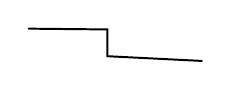
\begin{tikzpicture}[x=1mm,y=1mm,line cap=round]\draw[line width=.25mm] (0,3.5)--(10,3.4)--(10,0)--(22,-.6);\end{tikzpicture}}

, on retrouve $A(r)\leq B(r)$). Dans le cas actuel,

\[
A\deleted{\unsure{^{\,\prime}|{}^{\sim}}}(r)=\sum_1^n\log(1+r\rho_i(u))\qquad \text{donc }\ A'(r)=\sum\frac{r}{1+r\rho_i(u)}
\]

d'où notre assertion. Le cas le plus \deleted{\unsure{important}}\unsure{important} est celui où on prend $\varphi(r)=r^{-p}$ $0<p<1$. On trouve alors
\scanpage{76}
% archive sheet number: 77
\[
f_\varphi(\rho)=\rho^p\int\frac{s^{-p}}{1+s}\,ds=c^{\mathrm{te}}.\rho^p,
\]

d'où, en posant \deleted{\unsure{$S_p^{(n)}$|Système}} \unsure{a|a.}

\[
S_p^{(n)}(u)=\sum_1^n\rho_i(u)^p
\]

\[
S_p^{(n)}(u+v)\leq S_p^{(n)}(u)+S_p^{(n)}(v)
\]

en particulier

\[
S_p(u+v)\leq S_p(u)+S_p(v)
\]

\uline{\unsure{Remarque|Remarquons}} On a $\sum_1^n\rho_i(u+v)^p\leq\sum_1^n(\rho_i(u)+\rho_i(v))^p$, quel que soit $n$, on peut donc appliquer le lemme de Weyl ; on \unsure{trouve rien de spécial|trouve rien de spécial ?}

\figure{
\begin{tikzpicture}[x=1mm,y=1mm,line cap=round]\draw[gray,line width=.14mm] (9,23)..controls (12,28) and (15,25)..(13.6,22)..controls (12.5,19.8) and (3.5,15.5)..(1.7,8)..controls (-.9,-.3) and (2.3,-2.3)..(4.1,4.2)..controls (5.8,10.6) and (3.8,10.5)..(1.2,6.5)..controls (4.2,17) and (14.5,20.3)..(14.1,24.6);\end{tikzpicture}}

\uline{Question} Trouver la forme générale des fonctions $f$ d'une variable positive telle que, posant \deleted{\unsure{$S_f^{(n)}(u)$}} $f^{(n)}(u)=\sum_1^n\unsure{\rho_i(u)|f_i(u)|f(\rho_i(u))}$, on ait $f^{(n)}(u+v)\leq f^{(n)}(u)+f^{(n)}(v)$ quel que soit $n$. Il suffit qu'on ait $f^{\infty}(u+v)\leq f^{\infty}(u)+f^{\infty}(v)$

pour \deleted{\unsure{tout}}\unsure{tout} $u\in L(E)$, avec $E$ espace de Hilbert de dimension finie arbitraire. Généralisation à des fonctions de $n$ arguments.

\figure{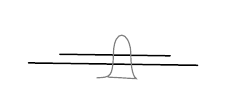
\begin{tikzpicture}[x=1mm,y=1mm,line cap=round]
\draw[line width=.19mm] (4,3)--(18,2.8) (0,1.9)--(21.5,1.6);
\draw[gray,line width=.15mm] (8.7,0).. controls (10.5,.1) and (10.7,.1)..(10.8,3.2)..controls (10.9,6.3) and (12.8,6)..(13,3.3)..controls (13,.8) and (13.4,.1)..(13.7,-.1)--(10.1,.1);
\end{tikzpicture}}
\scanpage{77}
% archive sheet number: 78
/ op. hermitiens positifs, enfin satisfait à la formule (12).

\margin{Mettre en tête 2 et corollaire}

\uline{Proposition 3} Soient $E$ et $F$ deux espaces de Hilbert, soient $u_i$ ($i=1,\ldots n$) des applications de Fredholm de $E$ dans $F$\unsure{;|,} alors $u_1\wedge\ldots\wedge u_n$ est une application de Fredholm de $\overset{n}{\Lambda}^{(2)}E$ dans $\overset{n}{\Lambda}^{(2)}F$, et

\[
\lVert u_1\wedge\ldots\wedge u_n\rVert_1\leq\frac1{n!}\lVert u_1\rVert_1\ldots\lVert u_n\rVert_1\tag*{(13)}
\]

En effet, il suffit de \deleted{\unsure{$\leq$}} vérifier \deleted{que si} si \deleted{$u_1=a_1\otimes$} $u_i=\bar b_i\otimes a_i$, \deleted{\unsure{les } \illegible{1}} avec $\lVert\bar b_i\rVert\leq1$, $\lVert a_i\rVert\leq1$, alors $\lVert u_1\wedge\ldots\wedgeu_n\rVert_1\leq1/n!$, \deleted{\unsure{car}} puisqu'alors il existe une application \unsure{de Banach|de forme} \unsure{linéaire|n-linéaire} \deleted{\unsure{continue}} \inserted{de norme $\leq1/n!$} de $(\bar E\widehat{\otimes}E)^n$ dans \deleted{\unsure{dans}} $\bar F\widehat{\otimes}F$ (où $F=\overset{n}{\Lambda}^{(2)}E$) qui coïncide avec \inserted{$(u_1,\ldots u_n)\longrightarrow$} $u_1\wedge\ldots\wedge u_n$ pour des $u_i$ décomposables, donc partout puisque les deux applications sont continues \deleted{\unsure{par}} en \deleted{\unsure{tant}} qu'applications dans $L(F)$.

Or pour $u_i=\bar b_i\otimes a_i$, on a \deleted{\unsure{$\overset{n}{\Lambda}$}}

\[
u_1\wedge\ldots\wedge u_n=\frac1{n!}(\bar b_1\wedge\ldots\wedge\bar b_n)\otimes(a_1\wedge\ldots\wedge a_n),
\]

\inserted{(voir Chap I, N\textsuperscript{o} 1, formule (8))} d'où

\[
\lVert u_1\wedge\ldots\wedge u_n\rVert_1\leq\frac1{n!}\lVert\bar b_1^{\unsure{i|c|'|{}}}\wedge\ldots\wedge\bar b_n\rVert\,\lVert a_1\wedge\ldots\wedge a_n\rVert\leq\frac1{n!}\prod\lVert a_i\rVert\,\lVert\bar b_i\rVert
\]

(formule (\unsure{5,|5}),), d'où (13).

\uline{Corollaire 1} Soit $E$ un espace de Hilbert, et \deleted{\unsure{$u$}}\inserted{$u,u_i$} $\in L^1(E)$ \deleted{\unsure{de Fredholm}} $(i=1,\ldots n)$ \deleted{des} opérateurs de Fredholm dans $E$. Alors $\overset{n}{\Lambda}u$ est un opérateur de Fredholm dans $\overset{n}{\Lambda}^{(2)}E$, et on a

\[
\deleted{\unsure{\text{alors}}}\ \deleted{\unsure{\alpha_n(u)}}\left\{\begin{aligned}
\alpha_n(u_1,\ldots,u_n)&=\operatorname{Tr}(u_1\wedge\ldots\wedge u_n)\\
\alpha_n(u)&=\operatorname{Tr}(\overset{n}{\Lambda}u)
\end{aligned}\right.\quad\text{en particulier}\tag*{(14)}
\]

(où $\alpha_n(u)$ est défini dans Chap 1, \S~2, prop 1) En effet, (14) est vraie \deleted{pour \unsure{tout}} quand on
\scanpage{78}
% archive sheet number: 79
est de rang fini \inserted{(vérifier d'après cas décomposable)} (voir Chap I, \S~1, N\textsuperscript{o} 2, définition 1), et reste donc vraie par \unsure{raison|raisons} de continuité dans le cas général. Conjointement avec (13), on trouve

\uline{Corollaire 2} Sous les conditions précédentes, on a

\[
|\alpha_n(u_1,\ldots u_n)|\leq\frac1{n!}\lVert u_1\rVert\ldots\lVert u_n\rVert\tag*{(15)}
\]

(Cela résulte aussi du fait, déjà \unsure{signalé}, que le coëfficient \unsure{$k_n$|$h_n$} du Chap I, \S~1, N\textsuperscript{o} 2, prop 1, est ici égal à 1).

\uline{Corollaire 3} Soit \deleted{$u\in L^1(E)$, où $E$ est un espace de Hilb} \inserted{\unsure{$u$ un} op. de Fredholm dans un} espace de Hilbert $E$. \deleted{Alors,} Si $u$ est un op. de Fredholm, il en est de même de $\overset{n}{\Lambda}u$, et on a

\[
\lVert\overset{n}{\Lambda}u\rVert_1=\alpha_n\deleted{\unsure{(\sqrt{u^*u})}}(|u|)=\alpha_n(\sqrt{\unsure{u^*u|u^*}})
\tag*{(16)}
\]

Si $u$ est un op. de H--S., il en est de même de $\overset{n}{\Lambda}u$, et on a

\[
\lVert\overset{n}{\Lambda}u\rVert_{\unsure{2|1}}=\sqrt{\alpha_n(u^*u)}\tag*{(\unsure{17|14})}
\]

On a, si $u\in L^1(E)$, $\lVert\overset{n}{\Lambda}u\rVert_1=\operatorname{Tr}\deleted{\unsure{\sqrt{\vphantom{(\overset{n}{\Lambda}u)^*}}}}\bigl((\overset{n}{\Lambda}u)^*(\overset{n}{\Lambda}u)\bigr)^{1/2}$ (N\textsuperscript{o} 1, formule (22)), or, (prop 1) on a $\deleted{\unsure{\sqrt{\vphantom{(\overset{n}{\Lambda}u)^*}}}}\bigl((\overset{n}{\Lambda}u)^*(\overset{n}{\Lambda}u)\bigr)^{1/2}=\overset{n}{\Lambda}\bigl((u^*u)^{1/2}\bigr)$, d'où \deleted{(16) en vertu de (17)} \inserted{$\lVert\overset{n}{\Lambda}u\rVert_1=\operatorname{Tr}\overset{n}{\Lambda}((u^*u)^{1/2})=\alpha_n(\sqrt{u^*u})$} (en vertu de (14)).

\deleted{Si $u\in L^2(E)$, \inserted{alors} on a encore $(\overset{n}{\Lambda}u)^*(\overset{n}{\Lambda}u)=\overset{n}{\Lambda}(u^*u)$ \unsure{où on} \unsure{avait} $u^*u\in L^1(E)$ \inserted{est op. de Fredholm} (d'où $(\overset{n}{\Lambda}u)^*(\overset{n}{\Lambda}u)=\overset{n}{\Lambda}(u^*u)$ est $\in L^1(E)$, et $\overset{n}{\Lambda}u$ \unsure{par suite}}

Si $u$ est un op. de H.--S., alors $u^*u$ est un op. de Fredholm (N\textsuperscript{o} 1, th.~4), donc $(\overset{n}{\Lambda}u)^*(\overset{n}{\Lambda}u)=\overset{n}{\Lambda}(u^*u)$ est un op. de Fredholm, \deleted{et} donc $\overset{n}{\Lambda}u$ est un op. de H.--S. On a (N\textsuperscript{o} 1, th.~3, corollaire 3)

\[
(\lVert\overset{n}{\Lambda}u\rVert_2)^2=\operatorname{Tr}(\overset{n}{\Lambda}u)^*(\overset{n}{\Lambda}u)=\alpha_n(u^*u)\qquad\text{(formule (14)) d'où (17)}.
\]
